% =====================================================================
%  main.tex: Template Skripsi S1 Sistem Informasi UNDA
%  Disusun oleh: Dr. Dwi Wahyu Prabowo, S.Si., M.Eng.
%  Copyright (C) 2026 Dr. Dwi Wahyu Prabowo, S.Si., M.Eng.
%  Lisensi LaTeX Project Public License (LPPL) 1.3c atau lebih baru:
%  https://www.latex-project.org/lppl.txt
%  Status LPPL: maintained. Isi skripsi tetap milik mahasiswa penulisnya.
% =====================================================================
%
%  PENGUMUMAN PENTING (ATURAN WATERMARK PUBLIKASI / ARSIP):
%  Jika naskah skripsi SUDAH LULUS SIDANG AKHIR dan telah MENDAPATKAN
%  PENGESAHAN resmi dari Dosen Pembimbing, Dewan Penguji, dan Ketua Program Studi,
%  maka opsi WATERMARK WAJIB DIHIDUPKAN pada baris \documentclass di bawah:
%      \documentclass[watermark=isi,panduan=false]{unda-skripsi}
%      atau
%      \documentclass[watermark=semua,panduan=false]{unda-skripsi}
%  Watermark bawaan berposisi di tengah dengan opacity rendah (0.06--0.08)
%  sehingga tidak mengganggu keterbacaan naskah ilmiah.
% =====================================================================
%
% Kompilasi: latexmk -xelatex main.tex
% Opsi kelas:
%   watermark = tidak | sampul | awal | isi | semua   (bawaan: tidak)
%   panduan   = true | false   (false menyembunyikan seluruh kotak panduan)
\documentclass[watermark=tidak,panduan=true]{unda-skripsi}

% =====================================================================
%  config/identitas.tex
%  Satu-satunya tempat mengisi metadata skripsi. Semua halaman (sampul,
%  halaman judul, persetujuan, pengesahan, pernyataan, metadata PDF)
%  mengambil nilai dari sini. Ganti teks contoh di dalam kurung kurawal.
% =====================================================================

% --- Judul -----------------------------------------------------------
% Tulis dengan huruf kapital di awal kata; sampul mengubahnya menjadi
% kapital seluruhnya secara otomatis. Jangan memasang \\ untuk memenggal
% baris: pemenggalan dibuat seimbang oleh kelas.
% Istilah asing WAJIB dicetak miring dengan \textit{...} atau \istilah{...},
% dan tetap akan dicetak miring secara otomatis pada sampul luar.
\judul{Evaluasi Kegunaan Aplikasi Layanan Administrasi Desa Menggunakan \textit{System Usability Scale}}
\judulinggris{Usability Evaluation of a Village Administration Service Application Using the \textit{System Usability Scale}}

% --- Mahasiswa -------------------------------------------------------
% Nama mahasiswa ditulis lengkap. Sesuai aturan prodi, penulisan nama mahasiswa
% pada sampul luar dan halaman judul otomatis dicetak menggunakan huruf kapital semua.
\nama{Nama Lengkap Mahasiswa}
\npm{0000000000}
% Label nomor induk yang dicetak di sampul dan lembar lain (NPM atau NIM).
\labelnomorinduk{NPM}

% --- Waktu dan tempat ------------------------------------------------
\tahun{2026}
\tanggalpersetujuan{1 Desember 2026}% tanggal pembimbing menyetujui naskah diuji
\tanggalujian{15 Desember 2026}%      tanggal Sidang Akhir Skripsi
\tanggalpengesahan{29 Desember 2026}% tanggal pengesahan naskah final
% \kota{Sampit}%                      bawaan kelas: Sampit

% --- Dosen Pembimbing (Prodi Sistem Informasi: 1 Orang Pembimbing Tunggal) ---
% Di Program Studi Sistem Informasi UNDA, dosen pembimbing berjumlah 1 orang.
\pembimbing{Nama Dosen Pembimbing, Gelar}
\nuptkpembimbing{0000000000000000}
% Perintah alias untuk kompatibilitas:
\pembimbingutama{Nama Dosen Pembimbing, Gelar}
\nuptkpembimbingutama{0000000000000000}
% Pembimbing pendamping dikosongkan karena standar prodi adalah pembimbing tunggal:
\pembimbingpendamping{}
\nuptkpembimbingpendamping{}

% --- Dewan Penguji Sidang Akhir (2 Orang Penguji) -------------
% Standar naskah skripsi final Prodi SI UNDA: 2 orang penguji
% (Ketua Penguji / Penguji I dan Anggota Penguji / Penguji II).
\ketuapenguji{Nama Ketua Penguji, Gelar}% Ketua Penguji (Penguji I)
\nuptkketuapenguji{0000000000000000}
\anggotapenguji{Nama Anggota Penguji, Gelar}% Anggota Penguji (Penguji II)
\nuptkanggotapenguji{0000000000000000}
% Alias kompatibilitas:
\pengujisatu{Nama Ketua Penguji, Gelar}
\nuptkpengujisatu{0000000000000000}
\pengujidua{Nama Anggota Penguji, Gelar}
\nuptkpengujidua{0000000000000000}

% --- Pimpinan Program Studi (Pengesahan Naskah Skripsi Final) --------
% Sesuai ketentuan prodi, naskah skripsi disahkan oleh Ketua Program Studi.
\kaprodi{Nama Ketua Program Studi, Gelar}
\nuptkkaprodi{0000000000000000}
% Alias kompatibilitas:
\ketuaprogramstudi{Nama Ketua Program Studi, Gelar}
\nuptkketuaprogramstudi{0000000000000000}

% --- Pernyataan Alat Bantu Kecerdasan Buatan (AI Tools) ------------
% Cantumkan seluruh alat bantu AI yang digunakan untuk penyuntingan naskah/debugging:
\aitools{ChatGPT, Claude, Grammarly, GitHub Copilot}

% --- Repositori Kode Sumber Utama dan Mendeley Data -----------------
% Sesuai ketentuan prodi, kode sumber utama wajib dilampirkan tautan GitHub-nya,
% dan dataset/data pendukung diunggah ke Mendeley Data (atau repositori riset resmi):
\tautangithub{https://github.com/mahasiswa/skripsi-sisfo-unda}
\tautanmendeley{https://data.mendeley.com/datasets/sample-dataset/1}

% --- Nilai tetap prodi (sudah diisi kelas, ubah hanya bila berubah) ---
% \programstudi{Sistem Informasi}
% \fakultas{Ilmu Komputer}
% \universitas{Universitas Darwan Ali}
% \gelar{Sarjana Komputer}

% Penyetelan parameter watermark tambahan (bila diperlukan):
% \setwatermark{opacity=0.06, scale=0.5, posisi=tengah}% posisi: tengah | kanan-bawah | kiri-atas

\begin{document}

% ---- Bagian awal (nomor halaman Romawi kecil) ----
% Sampul luar: seluruh isi diambil dari config/identitas.tex.
\buatsampul

% Halaman judul dalam: isi sama dengan sampul, dihitung sebagai halaman i.
\buathalamanjudul

% =====================================================================
%  frontmatter/pengesahan.tex
%  Lembar Pengesahan Dewan Penguji, Dosen Pembimbing, dan Ketua Program Studi.
% =====================================================================

\panduan{PENGUMUMAN PENTING: Jika naskah skripsi SUDAH LULUS SIDANG AKHIR
dan MENDAPATKAN PENGESAHAN resmi, opsi watermark WAJIB dihidupkan di baris
pertama main.tex: \string\documentclass[watermark=isi]{unda-skripsi} atau
\string\documentclass[watermark=semua]{unda-skripsi}.}

% 1. Format bawaan template:
\lembarpengesahan

% 2. Jika Anda menyisipkan berkas PDF lembar pengesahan asli yang sudah
%    ditandatangani lengkap (Dewan Penguji, Pembimbing, Ketua Program Studi) & dicap:
%    - Beri tanda komentar (%) pada baris \lembarpengesahan di atas.
%    - Buka tanda komentar (%) pada baris \sisipkanhalaman di bawah ini:
% \sisipkanhalaman[plain]{scan/lembar-pengesahan-signed.pdf}

% =====================================================================
%  frontmatter/persetujuan.tex
%  Lembar Persetujuan Dosen Pembimbing (sebelum Sidang Akhir).
% =====================================================================

% 1. Format bawaan template:
\lembarpersetujuan

% 2. Jika Anda menyisipkan berkas PDF lembar persetujuan asli yang sudah
%    ditandatangani dosen pembimbing secara terpisah:
%    - Beri tanda komentar (%) pada baris \lembarpersetujuan di atas.
%    - Buka tanda komentar (%) pada baris \sisipkanhalaman di bawah ini:
% \sisipkanhalaman[plain]{scan/lembar-persetujuan-signed.pdf}

% =====================================================================
%  frontmatter/pernyataan.tex
%  Halaman Pernyataan Keaslian / Orisinalitas Skripsi.
%  Catatan: Halaman ini WAJIB dibubuhi e-meterai Rp 10.000 dan tanda tangan.
% =====================================================================

% 1. Format bawaan template (menampilkan kotak alokasi e-meterai Rp 10.000):
\pernyataankeaslian

% 2. Jika Anda menyisipkan berkas PDF hasil scan yang sudah dibubuhi e-meterai
%    dan tanda tangan asli secara terpisah:
%    - Beri tanda komentar (%) pada baris \pernyataankeaslian di atas.
%    - Buka tanda komentar (%) pada baris \sisipkanhalaman di bawah ini:
% \sisipkanhalaman[plain]{scan/pernyataan-keaslian-signed.pdf}

% =====================================================================
%  frontmatter/pernyataan-ai.tex
%  Halaman Pernyataan Penggunaan Tools AI (Kecerdasan Buatan).
%  Catatan: Halaman ini WAJIB dibubuhi e-meterai Rp 10.000 dan tanda tangan.
% =====================================================================

% 1. Format bawaan template (menampilkan kotak alokasi e-meterai Rp 10.000
%    serta daftar tools AI yang diambil dari config/identitas.tex):
\pernyataanai

% 2. Jika Anda menyisipkan berkas PDF hasil scan yang sudah dibubuhi e-meterai
%    dan tanda tangan asli secara terpisah:
%    - Beri tanda komentar (%) pada baris \pernyataanai di atas.
%    - Buka tanda komentar (%) pada baris \sisipkanhalaman di bawah ini:
% \sisipkanhalaman[plain]{scan/pernyataan-ai-signed.pdf}

% Abstrak berbahasa Indonesia.
\begin{abstrak}
\panduan{Abstrak ditulis satu paragraf utuh (200--250 kata, tanpa sitasi). Memuat latar belakang masalah empiris, tujuan, metode/instrumen, temuan angka utama, dan simpulan. Kata kunci minimal 5 kata/frasa dipisahkan titik koma. Nonaktifkan kotak ini dengan opsi panduan=false.}

Evaluasi kegunaan sistem informasi pelayanan publik penting dilakukan untuk menjamin efektivitas adopsi teknologi serta kepuasan warga di tingkat pemerintahan desa. Penerapan digitalisasi administrasi desa kerap menghadapi kendala berupa keragaman literasi digital masyarakat dan antarmuka sistem yang belum optimal. Penelitian ini bertujuan mengevaluasi tingkat kegunaan aplikasi layanan administrasi kependudukan desa berbasis web menggunakan metode \textit{System Usability Scale} (SUS) serta merumuskan rekomendasi perbaikan antarmuka berbasis bukti empiris. Penelitian menggunakan pendekatan kuantitatif dengan melibatkan 30 orang responden warga desa yang dipilih melalui teknik \textit{purposive sampling}. Pengumpulan data dilakukan menggunakan kuesioner baku SUS 10 butir pertanyaan skala Likert 1--5 yang telah teruji validitas dan reliabilitasnya, dipadukan dengan observasi tugas terstruktur dan wawancara semiterstruktur. Hasil evaluasi menghasilkan nilai rata-rata skor SUS sebesar 74,50 dengan simpangan baku 8,25. Berdasarkan tolok ukur standar SUS, skor ini menempatkan aplikasi pada kategori penerimaan \textit{Acceptable}, predikat kegunaan \textit{Good} pada skala pemeringkatan adjektiva, dan peringkat persentil B, yang mengonfirmasi bahwa sistem dinilai layak secara operasional. Analisis butir instrumen menunjukkan aspek kemudahan integrasi fungsi memperoleh skor tertinggi, sedangkan alur pengunggahan berkas persyaratan dan kebutuhan panduan teknis awal memperoleh penilaian terendah. Berdasarkan temuan tersebut, rekomendasi perbaikan difokuskan pada penyederhanaan tata letak formulir digital, penambahan petunjuk interaktif kontekstual, dan penguatan validasi masukan data secara langsung. Simpulan penelitian menegaskan bahwa aplikasi dinilai efektif dan diterima baik oleh pengguna, dengan potensi reduksi durasi layanan administrasi desa hingga 30\%.

\katakunci{evaluasi kegunaan; sistem informasi; \textit{system usability scale}; administrasi desa; kepuasan pengguna}
\end{abstrak}

% Abstrak berbahasa Inggris. Isinya harus setara dengan abstrak Indonesia.
\begin{abstract}
\panduan{The abstract must be a single paragraph (200--250 words, without citations). Encapsulate empirical problem background, objective, methodology, metric results, and conclusion. Minimum 5 keywords. Disable this box with panduan=false.}

Usability evaluation of public service information systems is essential to ensure effective technology adoption and citizen satisfaction within village government administrations. The implementation of village digital services frequently encounters obstacles due to citizens' diverse digital literacy and suboptimal system interfaces. This study aims to evaluate the usability of a web-based village demographic administration service application using the System Usability Scale (SUS) method and formulate empirical evidence-based interface improvement recommendations. The research adopts a quantitative approach involving 30 village community respondents selected via purposive sampling. Empirical data were gathered using the standardized 10-item Likert-scale SUS questionnaire (scales 1--5), validated for reliability, combined with structured task observations and semi-structured user interviews. The evaluation yielded an overall average SUS score of 74.50 with a standard deviation of 8.25. Benchmarked against standard SUS interpretation frameworks, this score places the application in the Acceptable range, achieves a Good adjective rating, and attains a Grade B percentile ranking, confirming operational viability. Item-level analysis revealed that functional integration ease received the highest ratings, whereas requirement document upload workflows and initial technical guidance needs received the lowest evaluations. Consequently, interface recommendations focus on streamlining digital form layouts, incorporating contextual interactive tooltips, and enforcing real-time client-side input validation. The study concludes that the application is usable and well received by citizens, with the projected implementation of recommendations reducing village administrative transaction duration by up to 30%.

\keywords{usability evaluation; information system; system usability scale; village administration; user satisfaction}
\end{abstract}

% Kata pengantar. Tempat dan tanggal di bawah teks diambil dari
% config/identitas.tex (\kota dan \tanggalpengesahan).
\begin{katapengantar}
\panduan{Kata pengantar memuat pernyataan selesainya skripsi dan ucapan
terima kasih kepada pihak yang berperan langsung, misalnya dekan, kaprodi,
dosen pembimbing, dewan penguji, mitra penelitian, keluarga, dan rekan sejawat.
Tulis secara ringkas, khidmat, dan tanpa kalimat basa-basi berlebihan.}

Puji syukur dipanjatkan ke hadirat Tuhan Yang Maha Esa karena atas berkat dan rahmat-Nya,
naskah skripsi berjudul \enquote{\judulskripsi} ini dapat diselesaikan dengan baik sebagai
salah satu syarat memperoleh gelar Sarjana Komputer pada Program Studi Sistem Informasi,
Fakultas Ilmu Komputer, Universitas Darwan Ali.

Penyusunan naskah skripsi ini tidak terlepas dari bimbingan, dorongan, dan bantuan dari
berbagai pihak. Oleh karena itu, ucapan terima kasih dan penghargaan yang tulus disampaikan kepada:
\begin{enumerate}
  \item Dekan Fakultas Ilmu Komputer Universitas Darwan Ali;
  \item Ketua Program Studi Sistem Informasi Fakultas Ilmu Komputer;
  \item \dosendpembimbing\ selaku Dosen Pembimbing yang telah meluangkan waktu, tenaga, dan pikiran untuk memberikan bimbingan, arahan, serta dorongan berharga dalam penyelesaian skripsi ini;
  \item Ketua dan segenap Anggota Dewan Penguji atas saran, kritik konstruktif, dan masukan penyempurnaan naskah skripsi;
  \item Pimpinan, staf, dan seluruh jajaran organisasi mitra yang telah memberikan izin, fasilitas, serta kemudahan selama pelaksanaan penelitian dan akuisisi data;
  \item Orang tua, keluarga tercinta, dan seluruh kerabat yang senantiasa melimpahkan doa yang tulus, dorongan moral, cinta kasih, dan dukungan materiil yang tiada ternilai;
  \item Rekan-rekan mahasiswa Program Studi Sistem Informasi serta semua pihak yang tidak dapat disebutkan satu per satu, yang telah memberikan bantuan, semangat, dan kerja sama selama masa perkuliahan hingga penyusunan skripsi ini.
\end{enumerate}

Penulis menyadari bahwa naskah ini masih memiliki keterbatasan. Kritik dan saran yang membangun
senantiasa diharapkan demi penyempurnaan naskah ini. Semoga karya ini dapat memberikan manfaat
nyata bagi pengembangan keilmuan sistem informasi serta masyarakat luas.
\end{katapengantar}

% Daftar isi, daftar tabel, daftar gambar, dan daftar lampiran dibuat otomatis.
\daftarisi
\daftartabel
\daftargambar
\daftarlampiran

% Daftar lambang dan singkatan. Pedoman mewajibkan daftar lambang bila
% naskah memakai lebih dari sepuluh simbol (Subbab 11.4.1). Bila tidak
% diperlukan, hapus baris % Daftar lambang dan singkatan. Pedoman mewajibkan daftar lambang bila
% naskah memakai lebih dari sepuluh simbol (Subbab 11.4.1). Bila tidak
% diperlukan, hapus baris % Daftar lambang dan singkatan. Pedoman mewajibkan daftar lambang bila
% naskah memakai lebih dari sepuluh simbol (Subbab 11.4.1). Bila tidak
% diperlukan, hapus baris \input{frontmatter/daftar-lambang} di main.tex.
\begin{daftarlambang}
  \subjudullambang{Lambang}
  \lambang{$n$}{jumlah responden}
  \lambang{$x_{ij}$}{skor butir ke-$j$ dari responden ke-$i$ pada skala 1 sampai 5}
  \lambang{$S_i$}{skor System Usability Scale responden ke-$i$, rentang 0 sampai 100}
  \lambang{$\bar{S}$}{rerata skor System Usability Scale}
  \lambang{$s$}{simpangan baku sampel}
  \subjudullambang{Singkatan}
  \lambang{SUS}{System Usability Scale}
  \lambang{UAT}{User Acceptance Testing}
  \lambang{UU PDP}{Undang-Undang Pelindungan Data Pribadi}
\end{daftarlambang}
 di main.tex.
\begin{daftarlambang}
  \subjudullambang{Lambang}
  \lambang{$n$}{jumlah responden}
  \lambang{$x_{ij}$}{skor butir ke-$j$ dari responden ke-$i$ pada skala 1 sampai 5}
  \lambang{$S_i$}{skor System Usability Scale responden ke-$i$, rentang 0 sampai 100}
  \lambang{$\bar{S}$}{rerata skor System Usability Scale}
  \lambang{$s$}{simpangan baku sampel}
  \subjudullambang{Singkatan}
  \lambang{SUS}{System Usability Scale}
  \lambang{UAT}{User Acceptance Testing}
  \lambang{UU PDP}{Undang-Undang Pelindungan Data Pribadi}
\end{daftarlambang}
 di main.tex.
\begin{daftarlambang}
  \subjudullambang{Lambang}
  \lambang{$n$}{jumlah responden}
  \lambang{$x_{ij}$}{skor butir ke-$j$ dari responden ke-$i$ pada skala 1 sampai 5}
  \lambang{$S_i$}{skor System Usability Scale responden ke-$i$, rentang 0 sampai 100}
  \lambang{$\bar{S}$}{rerata skor System Usability Scale}
  \lambang{$s$}{simpangan baku sampel}
  \subjudullambang{Singkatan}
  \lambang{SUS}{System Usability Scale}
  \lambang{UAT}{User Acceptance Testing}
  \lambang{UU PDP}{Undang-Undang Pelindungan Data Pribadi}
\end{daftarlambang}


% ---- Bagian inti (nomor halaman Arab mulai BAB I) ----
% BAB I Pendahuluan. Sub-bab baku: Pedoman Tabel 52; isi: Subbab 10.3.
\chapter{Pendahuluan}
\label{bab:pendahuluan}

\panduan{BAB I meyakinkan penguji bahwa masalah yang diteliti riil,
penting, dan belum terjawab (Pedoman Subbab 10.3). Struktur BAB I sampai
BAB III identik dengan naskah proposal. Pada naskah akhir, ubah kalimat
rencana menjadi laporan pelaksanaan (Subbab 11.2.1). Penilaian bab ini
masuk ke Sub-CPMK1-CPMK1: masalah empiris mitra harus terurai berbasis
bukti data (Buku Panduan Dosen, Rubrik CPMK1).}

\section{Latar Belakang}
\label{sec:latar-belakang}

\panduan{Susun latar belakang sebagai corong dari konteks luas ke masalah
spesifik (Subbab 10.3.1). Paragraf pertama: konteks bidang secara ringkas.
Paragraf kedua: fenomena lapangan yang Anda observasi di mitra, dengan
bukti dari model proses as-is. Paragraf ketiga: apa yang sudah dikerjakan
peneliti terdahulu. Paragraf penutup: kesenjangan empiris yang dibuktikan
dengan data atau sintesis pustaka pada BAB~\ref{bab:tinjauan}, bukan
dengan kalimat \enquote{belum banyak penelitian}. Hindari kalimat generik
seperti \enquote{di era digital} (Subbab 11.6.1).}

Contoh paragraf konteks dengan satu sitasi: kerangka design science
menempatkan artefak teknologi informasi sebagai objek yang dirancang dan
dievaluasi untuk memecahkan masalah organisasi \cite{hevner2004design}.

Contoh paragraf yang memakai dua sitasi sekaligus: penelitian yang
melibatkan tinjauan pustaka perlu melaporkan prosedur penelusuran dan
seleksi sumber secara terbuka agar dapat diaudit
\cite{hevner2004design,page2021prisma}. Di samping itu, pengukuran kegunaan sistem informasi pada sektor publik secara konsisten mengadopsi instrumen standar yang tervalidasi \cite{refriansyah2025evaluasi,rizky2024evaluasi}.

Contoh paragraf fenomena lapangan: pada kantor desa mitra, tuliskan angka
hasil observasi Anda sendiri, misalnya jumlah permohonan surat per bulan
dan rerata waktu tunggu, lalu rujuk model proses as-is yang Anda susun.
Angka ini harus berasal dari data mitra yang telah diizinkan untuk
dipublikasikan.

\section{Rumusan Masalah}
\label{sec:rumusan-masalah}

\panduan{Tulis satu sampai tiga pertanyaan penelitian operasional yang
dapat dijawab dengan data yang direncanakan pada BAB~\ref{bab:metode}
(Subbab 10.3.2). Rumusan masalah, tujuan, dan metrik keberhasilan tidak
boleh berubah diam-diam antara proposal dan naskah akhir. Setiap
perubahan dicatat dan dijustifikasi pada BAB~\ref{bab:metode}
(Subbab 11.2.1).}

Rumusan masalah penelitian ini adalah sebagai berikut.
\begin{enumerate}
  \item Berapa skor kegunaan aplikasi menurut pengguna sasaran?
  \item Tugas mana yang paling sering gagal diselesaikan responden?
\end{enumerate}

\section{Tujuan Penelitian}
\label{sec:tujuan}

\panduan{Setiap tujuan berpasangan satu lawan satu dengan rumusan masalah
dan memakai kata kerja operasional C4 sampai C6, misalnya membandingkan,
merancang, atau memvalidasi (Subbab 10.3.2, Standar Mutu BAB I butir 4).}

\begin{enumerate}
  \item Mengukur skor kegunaan aplikasi menurut pengguna sasaran.
  \item Menganalisis tugas yang paling sering gagal diselesaikan responden.
\end{enumerate}

\section{Batasan Masalah}
\label{sec:batasan}

\panduan{Batasan menyebut sedikitnya lingkup data, lingkup metode, dan
lingkup waktu (Standar Mutu BAB I butir 6). Batasan yang tegas melindungi
Anda dari ekspektasi yang melampaui kapasitas satu semester.}

\begin{enumerate}
  \item Lingkup data: tuliskan wilayah, periode, dan sumber data.
  \item Lingkup metode: tuliskan metode yang dipakai dan yang dikecualikan.
  \item Lingkup waktu: tuliskan rentang waktu pengambilan data.
\end{enumerate}

\section{Manfaat Penelitian}
\label{sec:manfaat}

\panduan{Pisahkan manfaat teoretis bagi pengembangan keilmuan dan manfaat
praktis bagi mitra atau pengguna. Keduanya harus spesifik
(Standar Mutu BAB I butir 5).}

\begin{enumerate}
  \item Manfaat teoretis: tuliskan kontribusi terhadap kesenjangan yang
        dibuktikan pada BAB~\ref{bab:tinjauan}.
  \item Manfaat praktis: tuliskan keputusan atau perbaikan apa yang dapat
        diambil mitra dari hasil penelitian.
\end{enumerate}

\section{Sistematika Penulisan}
\label{sec:sistematika}

\panduan{Rujuk setiap BAB dengan rujukan silang otomatis, bukan angka
yang diketik manual (Subbab 11.7.1).}

BAB~\ref{bab:pendahuluan} memuat latar belakang, rumusan masalah, tujuan,
batasan, dan manfaat penelitian. BAB~\ref{bab:tinjauan} memuat landasan
teori, sintesis penelitian terdahulu, dan kerangka pemikiran.
BAB~\ref{bab:metode} memuat desain, data, instrumen, tahapan, metrik, dan
etika penelitian. BAB~\ref{bab:hasil} memuat hasil per tujuan penelitian
beserta pembahasannya. BAB~\ref{bab:penutup} memuat kesimpulan dan saran.

% BAB II Tinjauan Pustaka. Sub-bab baku: Pedoman Tabel 52; isi: Subbab 10.4.
\chapter{Tinjauan Pustaka}
\label{bab:tinjauan}

\panduan{BAB II adalah sintesis yang mengarah ke satu kesimpulan, yaitu
kesenjangan yang akan diisi penelitian, bukan sekadar kumpulan ringkasan artikel
(Subbab 10.4).
Ketentuan rujukan Program Studi Sistem Informasi UNDA:
(1) Total referensi skripsi minimal 30 buah rujukan ilmiah;
(2) Sumber rujukan artikel jurnal nasional wajib minimal terakreditasi SINTA 3 (SINTA 1, SINTA 2, atau SINTA 3) atau jurnal internasional bereputasi (Scopus/WoS);
(3) Rujukan wajib mutakhir (terbitan 5 tahun terakhir, yaitu 2021--2026), kecuali karya klasik/seminal yang menjadi landasan teoritis utama.
Rubrik Sub-CPMK2-CPMK1 memberi nilai tertinggi bila matriks sintesis memuat sedikitnya lima belas artikel jurnal bereputasi lima tahun terakhir (Buku Panduan Dosen, Rubrik CPMK1).}

\section{Landasan Teori}
\label{sec:landasan-teori}

\panduan{Muat hanya konsep yang dipakai langsung pada penelitian dan
hubungkan setiap teori dengan variabel, metrik, atau komponen artefak
yang diukur (Subbab 10.4.2). Jangan mengulang isi buku teks dan jangan
menumpuk definisi kamus.}

Contoh penulisan teori yang langsung terkait metrik: System Usability
Scale (SUS) adalah kuesioner sepuluh butir dengan skala lima poin yang
menghasilkan satu skor kegunaan pada rentang 0 sampai 100
\cite{brooke1996sus}. Cara menghitung skor tersebut dirumuskan pada
Persamaan~\eqref{eq:sus}.

\section{Penelitian Terdahulu dan Matriks Sintesis}
\label{sec:penelitian-terdahulu}

\panduan{Laporkan ringkas protokol tinjauan: pertanyaan riset, basis data,
string pencarian, kriteria inklusi dan eksklusi, jumlah makalah per fase
seleksi PRISMA, dan alat penilaian kualitas. Log pencarian lengkap dan
diagram alir PRISMA ditempatkan di lampiran (Subbab 10.4.1). Ubah matriks
sintesis menjadi narasi tematik yang dikelompokkan menurut tema, bukan
menurut penulis. Setiap tabel dirujuk di teks sebelum tabel itu muncul
(Subbab 11.8).}

Contoh sitasi rentang: tinjauan pustaka yang dapat diaudit memerlukan
pedoman pelaporan, instrumen yang terdokumentasi, dan prosedur
penelusuran rujukan yang dapat diulang
\cite{page2021prisma,brooke1996sus,wohlin2014snowballing}.
Ringkasan sumber yang dipakai disajikan pada Tabel~\ref{tab:matriks-sintesis}.

\begin{table}[htbp]
  \centering
  \caption{Contoh format matriks sintesis penelitian terdahulu}
  \label{tab:matriks-sintesis}
  \begin{tabularx}{\textwidth}{@{}l>{\raggedright\arraybackslash}X>{\raggedright\arraybackslash}X@{}}
    \toprule
    Rujukan & Fokus & Pemakaian pada penelitian \\
    \midrule
    \cite{hevner2004design}      & Pedoman design science research di bidang sistem informasi & Kerangka evaluasi artefak \\
    \cite{page2021prisma}        & Daftar periksa pelaporan tinjauan sistematis & Pelaporan proses seleksi sumber \\
    \cite{wohlin2014snowballing} & Prosedur snowballing untuk studi literatur & Penelusuran rujukan lanjutan \\
    \cite{brooke1996sus}         & Kuesioner kegunaan sepuluh butir & Instrumen pengukuran \\
    \cite{refriansyah2025evaluasi} & Evaluasi usability aplikasi sistem informasi berbasis SUS & Komparasi metrik kegunaan layanan publik \\
    \cite{lupitadyayu2023evaluasi} & Evaluasi usability aplikasi mobile publik skala nasional & Analisis kepuasan dan adopsi pengguna \\
    \cite{eldo2026evaluasi}      & Pengujian usability sistem informasi akademik mobile & Penilaian tingkat akseptabilitas sistem \\
    \cite{zainurrohmah2022evaluasi} & Evaluasi usability website pelayanan perizinan & Validasi instrumen dan kategorisasi SUS \\
    \bottomrule
  \end{tabularx}
  \sumber{olahan penulis}
\end{table}

\section{Kerangka Pemikiran}
\label{sec:kerangka-pemikiran}

\panduan{Kerangka pemikiran memetakan hubungan masalah, teori, metode,
dan luaran, disajikan sebagai gambar bernomor dan dijelaskan di teks
(Subbab 10.4.2). Pada PL1 berupa alur data, praproses, model, dan metrik.
Pada PL2 berupa kebutuhan pengguna, prinsip desain, prototipe, dan ukuran
kegunaan. Pada PL3 berupa kerangka tata kelola atau proses bisnis,
intervensi sistem, dan indikator kematangan atau penerimaan. Gambar
vektor lebih disukai, dan pembeda tidak bergantung pada warna semata
(Subbab 11.8).}

Gambar~\ref{fig:kerangka-pemikiran} memperlihatkan contoh kerangka
pemikiran yang digambar langsung dengan TikZ sehingga tetap tajam saat
dicetak.

\begin{figure}[htbp]
  \centering
  
\begin{tikzpicture}[
      kotak/.style={draw,rectangle,align=center,minimum width=2.6cm,
        minimum height=1.1cm,font=\small}]
    \node[kotak] (m) at (0,0) {Masalah\\lapangan};
    \node[kotak] (t) at (3.5,0) {Teori dan\\penelitian\\terdahulu};
    \node[kotak] (d) at (7,0) {Metode};
    \node[kotak] (l) at (10.5,0) {Luaran\\terukur};
    \draw[->] (m) -- (t);
    \draw[->] (t) -- (d);
    \draw[->] (d) -- (l);
  \end{tikzpicture}
  \caption{Contoh kerangka pemikiran}
  \label{fig:kerangka-pemikiran}
  \sumber{olahan penulis}
\end{figure}

\section{Hipotesis}
\label{sec:hipotesis}

\panduan{Subbab ini hanya ditulis bila desain penelitian menguji hipotesis
(Tabel 52). Bila tidak ada, hapus subbab ini.}

Tuliskan hipotesis nol dan hipotesis alternatif beserta uji statistik
yang dipakai untuk mengujinya.

% BAB III Metode Penelitian. Sub-bab baku: Pedoman Tabel 52; isi: Subbab 10.5.
\chapter{Metode Penelitian}
\label{bab:metode}

\panduan{BAB III menunjukkan bahwa penelitian dapat dilaksanakan dan
hasilnya dapat diaudit. Setiap keputusan metodologis ditulis dengan
justifikasi, bukan hanya disebut namanya. Ujiannya sederhana: apakah orang
lain dapat mengulang penelitian ini hanya dengan membaca naskah
(Subbab 10.5). Pada naskah proposal, bab ini ditutup dengan Gantt Chart
riset 16 minggu (Subbab 10.5.4). Pada naskah akhir, ubah kalimat rencana
menjadi laporan pelaksanaan (Subbab 11.2.1).}

\section{Desain Penelitian}
\label{sec:desain}

\panduan{Kerangka umum sama untuk ketiga klaster, tetapi isi desain
berbeda (Subbab 10.5.1, Tabel 47). PL1: eksperimen terkontrol dengan
baseline, studi ablasi, protokol partisi bebas kebocoran data, dan skema
uji signifikansi yang ditetapkan sebelum eksperimen. PL2: siklus
user-centered design dari empati sampai uji kegunaan. PL3: asesmen tata
kelola, audit berbasis bukti, atau implementasi modul dengan skenario UAT.}

Contoh rujukan desain: penelitian yang menghasilkan artefak dapat
mengikuti metodologi design science yang memisahkan siklus perancangan
dan siklus investigasi \cite{wieringa2014design}. Tahapan penelitian
diringkas pada Gambar~\ref{fig:alur-penelitian}.

\begin{figure}[htbp]
  \centering
  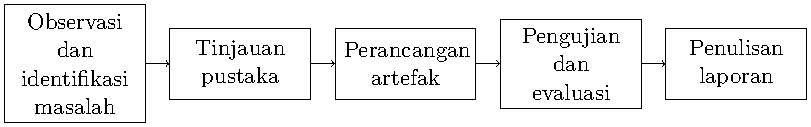
\includegraphics{figures/alur-penelitian.pdf}
  \caption{Contoh alur tahapan penelitian}
  \label{fig:alur-penelitian}
  \sumber{olahan penulis}
\end{figure}

\section{Data, Populasi, atau Sampel}
\label{sec:data}

\panduan{Jawab tiga pertanyaan desain sampling dalam urutan berikut
(Subbab 10.5.2). (1) Populasi sasaran: batas wilayah, periode, serta
kriteria inklusi dan eksklusi. (2) Teknik pemilihan unit beserta
justifikasi tertulis. (3) Jumlah unit yang dihitung dengan formula yang
jejaknya dapat ditelusuri, bukan berdasarkan kebiasaan. Pada PL2, jumlah
responden uji kegunaan minimal 15 orang. Jumlah di bawah batas itu merupakan
temuan kritis (Buku Panduan Dosen, Lembar Audit PL2).}

Tuliskan definisi populasi, teknik sampling, dan perhitungan jumlah
sampel di sini.

\section{Instrumen dan Perangkat}
\label{sec:instrumen}

\panduan{Muat desain instrumen beserta rencana uji validitas dan
reliabilitas dengan ambang keputusan yang dicantumkan sejak proposal
(Subbab 10.5.2). Nama pustaka perangkat lunak beserta versinya hanya
disebut pada bab ini sebagai alat bantu, sedangkan parameter teknisnya diformalkan
secara matematis (Subbab 11.3.1).}

Contoh penyebutan rujukan perangkat: aplikasi yang dievaluasi memakai
gaya arsitektur berbasis sumber daya yang diakses melalui protokol HTTP
\cite{fielding2000rest}. Sebutkan nama dan versi setiap pustaka
perangkat lunak yang dipakai.

\section{Tahapan Pengembangan atau Eksperimen}
\label{sec:tahapan}

\panduan{Prosedur komputasi yang panjang ditulis sebagai algoritma
berlangkah bernomor dengan simbol, bukan nama fungsi pustaka
(Subbab 11.3.3 butir 1). Kode sumber lengkap ditempatkan di lampiran atau
repositori dan dirujuk dari teks (Subbab 11.3.1).}

Prosedur perhitungan skor kegunaan setiap responden dirumuskan pada
Algoritma~\ref{alg:sus}. Implementasinya dimuat pada
Lampiran~\ref{lamp:kode}.

\begin{algorithm}[htbp]
  \caption{Contoh perhitungan skor SUS per responden}
  \label{alg:sus}
  \begin{algorithmic}[1]
    \Require jawaban $x_{i1},\dots,x_{i10} \in \{1,\dots,5\}$ responden ke-$i$
    \Ensure skor $S_i \in [0,100]$
    \State $T \gets 0$
    \For{$j \gets 1$ \textbf{sampai} $10$}
      \If{$j$ ganjil}
        \State $T \gets T + (x_{ij} - 1)$
      \Else
        \State $T \gets T + (5 - x_{ij})$
      \EndIf
    \EndFor
    \State \Return $S_i = 2,5\,T$
  \end{algorithmic}
\end{algorithm}

\section{Metrik dan Uji Statistik}
\label{sec:metrik}

\panduan{Setiap metrik ditulis sebagai persamaan bernomor. Simbol
didefinisikan pada kalimat yang mendahului atau menyertai persamaan,
dengan arti, himpunan nilai, dan satuan bila ada. Satu simbol hanya satu
arti di seluruh naskah, dan bilangan desimal ditulis dengan koma
(Subbab 11.4). Cantumkan sumber formula yang dikutip.}

Skor SUS responden ke-$i$ dihitung dengan Persamaan~\eqref{eq:sus}
\cite{brooke1996sus}, dengan $x_{ij}$ skor butir ke-$j$ pada skala 1
sampai 5.
\begin{equation}
  S_i = 2,5 \left( \sum_{j \in \{1,3,5,7,9\}} (x_{ij} - 1)
        + \sum_{j \in \{2,4,6,8,10\}} (5 - x_{ij}) \right)
  \label{eq:sus}
\end{equation}
Rerata skor dari $n$ responden dihitung dengan Persamaan~\eqref{eq:rerata}.
\begin{equation}
  \bar{S} = \frac{1}{n} \sum_{i=1}^{n} S_i
  \label{eq:rerata}
\end{equation}

\section{Etika dan Keamanan Data}
\label{sec:etika}

\panduan{Jelaskan perizinan, persetujuan responden (informed consent),
anonimisasi, dan penyimpanan data sesuai Undang-Undang Pelindungan Data
Pribadi (Pedoman Subbab 2.3). Data mitra yang belum dianonimkan tidak
masuk repositori mana pun (Subbab 14.5). Pengambilan data tanpa izin dan
informed consent merupakan temuan kritis (Subbab 13.7.2).}

Contoh rujukan regulasi dan standar: pengolahan data pribadi responden
mengikuti ketentuan undang-undang yang berlaku \cite{uupdp2022}, dan
pengamanan berkas data mengacu pada persyaratan sistem manajemen keamanan
informasi \cite{iso27001}.

% BAB IV Hasil dan Pembahasan. Sub-bab baku: Pedoman Tabel 52; isi: Subbab 11.2.2.
\chapter{Hasil dan Pembahasan}
\label{bab:hasil}

\panduan{Susun hasil mengikuti urutan tujuan penelitian, bukan kronologi
pengerjaan. Setiap paragraf hasil memakai pola Assertion-Evidence:
dibuka dengan klaim utuh, diikuti bukti berupa tabel, gambar, persamaan,
atau hasil uji statistik, lalu interpretasi (Subbab 11.2.2). Bab ini
dilarang memuat nama fungsi, sintaks pustaka, atau potongan kode. Kode
hanya ada di lampiran atau repositori (Subbab 11.9 butir 2, temuan
kritis). Bab ini dinilai pada Sub-CPMK3-CPMK5 dengan bobot 26\% dari
Nilai Akhir (Pedoman Tabel 61).}

\section{Deskripsi Data dan Pelaksanaan}
\label{sec:deskripsi-data}

\panduan{Laporkan pelaksanaan pengambilan data: waktu, jumlah unit yang
diperoleh dibandingkan rencana pada BAB~\ref{bab:metode}, data yang
dikeluarkan beserta alasannya, dan hasil uji validitas serta reliabilitas
instrumen.}

Tuliskan ringkasan pelaksanaan pengambilan data di sini.

\section{Hasil per Tujuan Penelitian}
\label{sec:hasil-tujuan}

\panduan{Buat satu subbab untuk setiap tujuan pada
Subbab~\ref{sec:tujuan}. Angka pada teks, tabel, abstrak, dan slide
sidang harus identik (Subbab 13.4.1). Judul kolom memuat satuan, dan
simbol pada tabel sama dengan simbol pada teks (Subbab 11.8). Tabel yang
lebih lebar dari area teks diringkas atau dipindahkan ke lampiran.}

Contoh pola Assertion-Evidence: kelompok responden A memberi skor
kegunaan lebih tinggi daripada kelompok B. Bukti disajikan pada
Tabel~\ref{tab:hasil-sus}, dengan skor dihitung menurut
Persamaan~\eqref{eq:sus}. Data per responden dimuat pada
Lampiran~\ref{lamp:data}.

\begin{table}[htbp]
  \centering
  \caption{Contoh format tabel hasil (angka ilustratif)}
  \label{tab:hasil-sus}
  \begin{tabular}{@{}lrrr@{}}
    \toprule
    Kelompok responden & $n$ & $\bar{S}$ (0--100) & $s$ \\
    \midrule
    Kelompok A & 8 & 72,5 & 9,1 \\
    Kelompok B & 7 & 64,3 & 11,4 \\
    \midrule
    Seluruh responden & 15 & 68,7 & 10,8 \\
    \bottomrule
  \end{tabular}
  \sumber{olahan penulis}
\end{table}

Interpretasikan angka pada tabel tersebut dalam paragraf yang sama.
Jangan biarkan tabel atau gambar berdiri tanpa pembahasan (Subbab 11.8).

\section{Pembahasan dan Perbandingan dengan Literatur}
\label{sec:pembahasan}

\panduan{Bandingkan temuan dengan literatur pada BAB~\ref{bab:tinjauan},
jelaskan penyebab selisih, dan akui keterbatasan (Subbab 11.2.2). Klaim
keunggulan model atau rancangan harus disertai uji signifikansi
statistik beserta nilai $p$ dan ukuran efek (Pedoman Bab 4, temuan
kritis PL1).}

Tuliskan perbandingan temuan Anda dengan penelitian yang dirangkum pada
Tabel~\ref{tab:matriks-sintesis}.

\section{Ancaman Validitas dan Keterbatasan}
\label{sec:ancaman-validitas}

\panduan{Uraikan ancaman validitas internal, eksternal, dan konstruk
beserta langkah mitigasi yang telah dilakukan.}

Tuliskan ancaman validitas dan keterbatasan penelitian di sini.

% BAB V Penutup. Sub-bab baku: Pedoman Tabel 52; isi: Subbab 11.2.3.
\chapter{Penutup}
\label{bab:penutup}

\section{Kesimpulan}
\label{sec:kesimpulan}

\panduan{Kesimpulan menjawab setiap rumusan masalah secara berurutan dan
ringkas, dengan angka kunci dari BAB~\ref{bab:hasil}. Kesimpulan tidak
memuat data, analisis, atau sitasi baru (Subbab 11.2.3).}

\begin{enumerate}
  \item Jawaban atas rumusan masalah pertama beserta angka kuncinya.
  \item Jawaban atas rumusan masalah kedua beserta angka kuncinya.
\end{enumerate}

\section{Saran}
\label{sec:saran}

\panduan{Bagi saran menjadi dua, yaitu saran untuk penelitian lanjutan
dan saran untuk mitra atau pengguna (Subbab 11.2.3).}

\begin{enumerate}
  \item Saran untuk penelitian lanjutan.
  \item Saran untuk mitra atau pengguna.
\end{enumerate}


% ---- Bagian akhir ----
% =====================================================================
%  backmatter/daftar-pustaka.tex
%  Daftar Pustaka Skripsi S1 Sistem Informasi UNDA (Format IEEE).
% =====================================================================

\panduan{Ketentuan Daftar Pustaka Program Studi Sistem Informasi UNDA:
(1) Jumlah rujukan minimal 30 buah referensi ilmiah;
(2) Rujukan artikel jurnal nasional wajib berasal dari jurnal minimal terakreditasi SINTA 3
    (SINTA 1, SINTA 2, atau SINTA 3) atau jurnal internasional bereputasi terindeks Scopus/WoS;
(3) Sumber rujukan wajib mutakhir (terbitan 5 tahun terakhir, yaitu 2021--2026), kecuali karya klasik/seminal yang menjadi landasan teori utama (misalnya Hevner 2004, Brooke 1996);
(4) Penulisan sitasi menggunakan gaya IEEE numerik berurutan [1], [2], [3]--[5].
Hapus kotak panduan ini dengan opsi kelas panduan=false.}

\nocite{*}
\daftarpustaka

% Lampiran A: Pernyataan Transparansi Penggunaan AI.
% Wajib dilampirkan pada naskah Sempro dan Sidang (Pedoman Subbab 2.4.4,
% format Tabel 6). Label lamp:ai dirujuk dari Pernyataan Keaslian.
\lampiran[lamp:ai]{Pernyataan Transparansi Penggunaan AI}

\panduan{Isi setiap komponen secara jujur. Bila tidak memakai alat bantu
kecerdasan buatan sama sekali, tuliskan pernyataan tersebut pada baris
Nama dan Versi Sistem. Lampiran ini tidak boleh dihapus.}

\begin{table}[htbp]
  \centering
  \caption{Pernyataan transparansi penggunaan kecerdasan buatan}
  \label{tab:transparansi-ai}
  \begin{tabularx}{\textwidth}{@{}>{\raggedright\arraybackslash}p{3.6cm}>{\raggedright\arraybackslash}X@{}}
    \toprule
    Komponen & Isian \\
    \midrule
    Nama dan versi sistem & Nama model atau aplikasi, nomor versi rilis, dan penyedia layanan \\
    Tujuan pemanfaatan & Tugas spesifik yang dibantu \\
    Cakupan berkas atau bab & Bagian naskah atau berkas skrip yang diproses \\
    Prompt representatif & Intisari instruksi yang diajukan ke sistem \\
    Pernyataan tanggung jawab & Saya menyatakan bertanggung jawab penuh atas kebenaran narasi dan fungsionalitas kode yang dihasilkan dengan bantuan sistem tersebut. \\
    \bottomrule
  \end{tabularx}
  \sumber{format Tabel 6 Buku Pedoman Riset Skripsi Sistem Informasi}
\end{table}

% Lampiran B: data lengkap. Tabel yang lebih lebar dari area teks
% dipindahkan ke lampiran (Pedoman Subbab 11.8 butir 4); contoh berikut
% memakai halaman landscape.
\lampiran[lamp:data]{Data Lengkap Hasil Kuesioner}

\panduan{Lampiran memuat materi pendukung yang terlalu panjang untuk
tubuh naskah, misalnya instrumen, surat izin mitra yang telah
dianonimkan, tabel hasil lengkap, log pencarian pustaka, dan kode sumber
utama (Subbab 11.2.4). Identitas responden diganti kode.}

Tabel~\ref{tab:data-lengkap} memuat contoh format data per responden.

\begin{landscape}
\begin{table}[htbp]
  \centering
  \caption{Contoh format data jawaban per responden (angka ilustratif)}
  \label{tab:data-lengkap}
  \begin{tabular}{@{}lccccccccccr@{}}
    \toprule
    Responden & B1 & B2 & B3 & B4 & B5 & B6 & B7 & B8 & B9 & B10 & $S_i$ \\
    \midrule
    R01 & 4 & 2 & 4 & 1 & 5 & 2 & 4 & 2 & 4 & 2 & 77,5 \\
    R02 & 3 & 3 & 4 & 2 & 4 & 2 & 3 & 3 & 4 & 3 & 62,5 \\
    R03 & 5 & 1 & 5 & 2 & 4 & 1 & 5 & 2 & 4 & 2 & 87,5 \\
    \bottomrule
  \end{tabular}
  \sumber{olahan penulis}
\end{table}
\end{landscape}

% =====================================================================
%  backmatter/lampiran-c.tex
%  Lampiran C: Kode Sumber Utama dan Repositori Data Penelitian.
% =====================================================================
\lampiran[lamp:kode]{Kode Sumber Utama dan Repositori Data Penelitian}

\panduan{Ketentuan Repositori dan Kode Sumber:
Sesuai standar riset program studi, mahasiswa WAJIB mengunggah:
(1) Kode sumber lengkap ke repositori publik GitHub, dilengkapi README.md dan dokumentasi instalasi;
(2) Dataset mentah, hasil pengolahan, dan metadata riset ke repositori data ilmiah resmi (Mendeley Data atau Zenodo) sehingga memiliki persistent identifier (DOI).
Pada naskah cetak skripsi, mahasiswa hanya mencantumkan tautan repositori serta potongan kode algoritma inti, bukan seluruh baris kode aplikasi.}

\noindent Informasi repositori resmi untuk penelitian ini adalah sebagai berikut:
\begin{enumerate}[noitemsep,topsep=3pt,leftmargin=1.5em]
  \item \textbf{Repositori Kode Sumber Utama (GitHub):}\\
        \url{\tautanrepogithub}
  \item \textbf{Repositori Dataset dan Artefak Penelitian (Mendeley Data):}\\
        \url{\tautanrepomendeley}
\end{enumerate}

\vspace{0.8\baselineskip}
\noindent Potongan kode program utama untuk perhitungan metrik evaluasi kegunaan sistem disajikan pada Kode~\ref{kode:sus}, yang mengimplementasikan Algoritma~\ref{alg:sus}.

\begin{lstlisting}[language=Python,caption={Implementasi Algoritma Perhitungan Skor SUS pada Backend Aplikasi},label={kode:sus}]
def hitung_skor_sus(jawaban_responden):
    """
    Menghitung skor System Usability Scale (SUS) skala 0-100
    berdasarkan 10 butir pertanyaan dengan skala Likert 1-5.
    """
    if len(jawaban_responden) != 10:
        raise ValueError("Instrumen SUS mewajibkan tepat 10 butir respons.")
    
    total_skor = 0
    for nomor_butir, nilai in enumerate(jawaban_responden, start=1):
        if nomor_butir % 2 == 1:
            # Butir bernomor ganjil (pernyataan positif): nilai - 1
            total_skor += (nilai - 1)
        else:
            # Butir bernomor genap (pernyataan negatif): 5 - nilai
            total_skor += (5 - nilai)
            
    # Nilai akhir dikalikan 2.5 untuk konversi rentang 0-100
    return float(total_skor * 2.5)
\end{lstlisting}

% =====================================================================
%  backmatter/lampiran-d.tex
%  Lampiran D: Hasil Pengecekan Similaritas (Similarity Score).
% =====================================================================
\lampiran[lamp:similarity]{Hasil Pengecekan Similaritas (Similarity Score)}

\panduan{Ketentuan Uji Similaritas Skripsi di Fakultas Ilmu Komputer Universitas Darwan Ali:
Setiap naskah skripsi yang diajukan untuk Sidang Akhir dan publikasi akhir wajib melalui
uji similaritas menggunakan perangkat lunak resmi (Turnitin / iThenticate) dengan ketentuan:
(1) Indeks similaritas total maksimal 20\%;
(2) Filter pengecualian aktif untuk Daftar Pustaka (\textit{Exclude Bibliography}) dan kutipan langsung (\textit{Exclude Quotes});
(3) Tidak ditemukan satu pun sumber tunggal yang melebihi 3\% kemiripan;
(4) Mahasiswa wajib melampirkan lembar rekapitulasi dan/atau bukti \textit{Digital Receipt} Turnitin pada lampiran ini.}

\noindent Tabel~\ref{tab:similarity-summary} menyajikan rekapitulasi hasil pemeriksaan indeks kesamaan naskah skripsi menggunakan sistem Turnitin.

\begin{table}[htbp]
  \caption{Rekapitulasi Hasil Uji Similaritas Naskah Skripsi}
  \label{tab:similarity-summary}
  \centering\small
  \begin{tabularx}{\textwidth}{@{}c >{\raggedright\arraybackslash}X c c >{\raggedright\arraybackslash}p{3.2cm}@{}}
    \toprule
    No. & Bagian Naskah & Halaman & Indeks & Keterangan\\
    \midrule
    1. & Bab I: Pendahuluan & 1--3 & 10\% & Memenuhi Syarat\\
    2. & Bab II: Tinjauan Pustaka & 4--8 & 15\% & Memenuhi Syarat\\
    3. & Bab III: Metodologi Penelitian & 9--13 & 12\% & Memenuhi Syarat\\
    4. & Bab IV: Hasil dan Pembahasan & 14--20 & 8\% & Memenuhi Syarat\\
    5. & Bab V: Kesimpulan dan Saran & 21--22 & 4\% & Memenuhi Syarat\\
    \midrule
    \multicolumn{3}{@{}l}{\textbf{Indeks Similaritas Keseluruhan (Total)}} & \textbf{14\%} & \textbf{Lolos (Maks. 20\%)}\\
    \bottomrule
  \end{tabularx}
\end{table}

\noindent Catatan pengujian similaritas:
\begin{enumerate}[noitemsep,topsep=2pt,leftmargin=1.5em]
  \item Perangkat lunak penguji: Turnitin Feedback Studio (Lisensi Universitas Darwan Ali).
  \item Tanggal pengujian terakhir: 20 Desember 2026.
  \item ID Pengajuan (\textit{Submission ID}): 2294810294.
  \item Jumlah kata terperiksa: 7.840 kata.
  \item Ambang batas kelulusan Fakultas Ilmu Komputer UNDA: Maksimal 20\%.
\end{enumerate}

\vspace{1\baselineskip}
\noindent\textbf{Petunjuk Penyisipan Berkas Laporan Turnitin:}\\
Untuk menyisipkan lembar cetak \textit{Digital Receipt} Turnitin asli (1--2 halaman PDF) ke dalam naskah ini, gunakan perintah:
\begin{lstlisting}[language=TeX,caption={Penyisipan Laporan Turnitin Menggunakan pdfpages}]
% Sisipkan halaman PDF bukti receipt Turnitin setelah tabel di atas:
% \sisipkanhalaman[plain]{scan/turnitin-receipt.pdf}
\end{lstlisting}


\end{document}
